
\documentclass[11pt,letterpaper]{article}
\usepackage{naaclhlt2016}
\usepackage{times,hyperref,latexsym,graphicx,listings,wrapfig,float,dcolumn,epsf,amsmath,widetext}

\naaclfinalcopy % Uncomment this line for the final submission
\def\naaclpaperid{***} %  Enter the naacl Paper ID here


\newcommand\BibTeX{B{\sc ib}\TeX}


\title{Reducing Packet Filtering Rules via K-Means Clustering}

\author{Max Bass \and Prof. Balajee Vanaman}


\date{}

\begin{document}

\maketitle

\begin{abstract}
This project originally aimed to increase packet filtering efficiency and reduce rule storage overhead by  combining overlapping and duplicate rules. Rules were clustered and combined via a k-means clustering algorithm. It was revealed that for short rule lists, the error from this method is impractically high, because rules are much farther apart in feature space than they are wide. The failure of clustering due to rule rule sparseness within ipv4 address space suggests a much bigger failure of clustering methods with rules in ipv6 address space, which is much larger. However, it was also found that in the averaged case, for certain stretches, the increase in error is minimal, as the rule number is decrease. This suggests potential effectiveness of clustering for rule reduction on a sufficiently large rule list, with a good heuristic.
\end{abstract}


\section{Intro and Background}

\subsection{motivation}
Packet filtering occurs at many different layers of a network, and especially prominently in core network infrastructure, and in datacenters. It is important for netork security, quality of service, and network analysis. Efficiency and efficacy is key. Small differences in run times lead to large differences in power consumption and performance over time.

Packet filtering using a decision tree ideally has an average run time of O(log(n)) per packet flow, where n is the length of the list of rules for a packet to be filtered through. In practice, this run time often approaches O(n) time. There is also some memory overhead from rule duplication in the tree, which occurs in efficuts [1] by a factor of 1.5, and in previous implementations like hypercuts and hicuts [4,5] by factors on the order of 50. 


\subsection{previous work}
Most other related to packet filtering uses decision trees, but {\bf not} trees constructed using Id3, C4.5, information gain, or informational entropy as heuristics. Rather, they split on relative density of rules in rule space. [1,4,5]

\subsection{where this project fits in}
While there has been much work on predicting different aspects of packet classification (maliciousness, type of service, and other label-able characteristics of packets, there hasn't been much work (that this author could find) that used unsupervised learning to optimize network policies. Hence, k-means clustering was used to investigate the reduction of rule duplication, which has been a necessary byproduct of previous packet filtering techniques [1,4,5]. 

\section{Methods}
\subsection{Machine Learning Formalism}
This subsection aims to formally define the machine learning terms for this problem.
{\bf Instances}: From the perspective of the algorithm, each instance is a packet filtering rule.
\newline
{\bf features}: There are eight features used per instance: "srcIPstart", "srcIPend", "dstIPstart","dstIPend", "srcPortStart", "srcPortEnd", "dstPortStart","dstPortEnd"

Each rule has a source and destination ip range and port range. The port ranges are specified in the input files by a start port and an end port. The ip ranges are specified in the input files by an ip address and mask, from which a start ip address and an end ip address can be obtained. Each ip address is in ipv4 format, hence is of the form "a.b.c.d", where a,b,c,d are each numbers between 0 and 255. This project's implementation of the algorithm treats each of these features as real numbers, rather than as 32 boolean features per ip address.
\newline \newline
{\bf feature space} this consists of all possible ranges of source and destination ip address and port. There are $2^{32}$ possible start and end ip addresses, and $2^{16}$ possible start and end ports. The start ip must be a lower number than the end ip, and the start port must be a lower number than the end port. Both ip addresses and ports can only be integers in their respective ranges.
\newline \newline
{\bf solution} A particular solution is a list of rules, specified by clusters, which each contain some set of rules. The rule specified by a cluster encompasses all of its rules in feature space. 
\newline \newline
{\bf solution space}: all possible clusters. Since all rules must pertain to a cluster, and clusters are defined by their rules, the set of all possible clusters is all combinations of rules. 
\newline \newline
{\bf learning algorithm}: A simple k-means clustering algorithm was used. Nearest boarder was also implemented, but not used, due to the time needed to test being more than the time available. The algorithm is polynomial in m (number of rules/instances), but still on the order of hours for multiple files of 5000 rules. Each cluster represents a hyperrectangular rule that encompasses the set of rules pertaining to it. 
\subsection{pipeline}
Raw data was generated in class bench, reformatted via bash scripting. From these reformatted files, features were extracted by a feature extraction java file to weka-specific arff files. These arff files were each read by a java program which did the clustering, and analyzed various measures of accuracy at each step, and then output the results to csv files. The csv files were read, aggregated, and graphed by a matlab program. All relevant data is publicly available in the repository \url{https://github.com/maxthefirstborn/cs446fall2016project}

\subsection{code}
The clustering algorithm was written in java, using instances in the weka framework. Weka was also used to extract the features from raw text files with lists of packet filtering rules. The java code outputs a comma separated value text file, which lists the total number of clusters in decreasing order (as the k-means clustering algorithm progresses), alongside certain error heuristics: the total error, which is just the hypervolume of all of the clusters, minus the total hypervolume of all of the rules. This quantity corresponds to they hypervolume in feature space in which a packet would be classified as falling into a rule, where it shouldn't. In other words, there are no false negative packet classifications in this model, only false positives, but a fairly high proportion of them. 
\subsection{data}
The text files analyzed were generated by classbench [6]. There were three categories of rule sets, associated with three different types of actions on packets, related to access control (acl), forwarding (fw), and interprocess communication (ipc). However, the distribution of rules is independent of the rule's action category, so for the purposes of this project, all rules sets are treated equally. 

\section{Results}
See graphs in appendix. Most notable among each set of graphs is the bottom left: $log_{10} (\frac{d Error}{d cluster size})$. Particularly, there are multiple plateaus  in almost all of the graphs, and most notably in the averaged case. This suggests that clustering is, in fact, in the average case, somewhat effective at combining overlapping rules

There is the change in error per iteration of the algorithm (per decrease in cluster size). There is a heuristic cost function, which is the product of the cluster size (total number of rules) and the error. This function increases exponentially as cluster size increases, so it turns out to be a terrible heuristic to optimize for, which went against the original assumptions. There is also the log of the change in error per iteration.

\section{Analysis and Discussion}
The result that the rules each specify ip ranges much smaller than the areas between each rule has implications about future potential approaches. Rule reduction by clustering worked by combining rules so that the space in between them was included in the new rule. In the results, it was found that rule combination in such a fashion is impractical, because even in the case of ipv4 addresses, which have an address space of $2^{32}\approx 4.3x 10^9$, the rule density an any particular area in the feature space was not nearly enough to justify combining.

The ipv6 addressing scheme has an address space of $2^{128} \approx 3.4x10^{38}$ , which is far beyond that of the address space for ipv4 (bigger by a factor of $2^{96} \approx 7.9x10^{28}$ ). Furthermore, because of the choices of ipv6 reserved address ranges, as specified by RFC 4291, as well as by probability that given a wider address space, a wider address space will be used, packet filtering rules for ipv6 addressed packets will likely be much more disperse than those for ipv4. 

However, one interesting thing to note about the k-means algorithm is that the $\frac{d Error}{d iteration}$ is zero for many steps, even though error-space minimization was {\bf not} used as a heuristic for the clustering algorithm. This promises potential usefulness for a clustering algorithm that were to take advantage of such a heuristic. 

\section{Conclusion}
Combining packet filtering rules via k-means clustering, without additional heuristics, often produces aggregate rules with impractically large inaccuracy, because the rule hypervolumes in feature space are much smaller than the distances between rules in rule space. However, in the average (aggregated) case, it was found that within certain thresholds, for a sufficiently long list of rules


\section{Future Work}
The main finding of this project is that packet filtering rules in a feature space defined by ip and port ranges are sparse. The hypervolume in feature space occupied by the rules is much smaller than the hypervolume between many of the rules. An approach could be used that takes advantage of rule sparseness in feature space.

For instance, rather than treating each feature, as described in the formalism section, as a real number, the features could each be treated as a set of boolean features. Thus, an ip start and end would each be specified by 32 boolean features, and a port start and end would each be specified by 16 boolean features. Thus, there would be 32 + 32 + 32 + 32 + 16 + 16 + 16 + 16 = 192 boolean features. If ipv6 addresses were used instead of ipv4 addresses, there would be 128 + 128 + 128 + 128 + 16 + 16 + 16 + 16 = 576 boolean features. Then, an algorithm like winnow, or SVM could potentially be used to learn good split points in a decision tree. 

If it was instead the case that clustering was found to have much higher accuracy, as was anticipated, then the next step would have been to use a more generalized form of clustering on the data: clustering via decision tree: a CLTree [3]. If the results of this project are found to be invalid, or inapplicable to certain cases, then a CLTree would be a good generalization of the clustering strategy. It is more difficult to implement than a simple k-means clustering algorithm, but it provides the advantage of naturally finding an optimal number of clusters. This is important because while in two or even three dimensional space an optimal number of clusters to pick is intuitive, in higher dimensions, and with sparser and more uniform data, it is not, and relies heavily on the dataset. Tree clusters, on the other hand, provides a heuristic purity function that performs consistently, for any dataset. 

\begin{widetext}
\section*{Acknowledgments}

Prof. Balajee Vanaman, for suggesting the approach to treat all rules as if they had the same action. Given this, rule priority becomes irrelevant, and packet filtering becomes a question of whether a packet falls into the space defined by {\bf any } rule in a rule list. Also, for providing the dataset, which was generated by classbench. 

\section{resources and references}
\begin{enumerate}
\item Balajee Vamanan, Gwendolyn Voskuilen, and T.N. Vijaykumar, “EffiCuts: Optimizing Packet Classification for Memory and Throughput,” in Proceedings of the ACM SIGCOMM Conference on Applications, Technologies, Architectures, and Protocols for Computer Communication (SIGCOMM), 2010.
\item W. Li and A. W. Moore, "A Machine Learning Approach for Efficient Traffic Classification," 2007 15th International Symposium on Modeling, Analysis, and Simulation of Computer and Telecommunication Systems, Istanbul, 2007, pp. 310-317.
doi: 10.1109/MASCOTS.2007.2
\item "Clustering via Decision Tree Construction", (with B. Liu, and Y. Xia), in Foundations and Advances in Data Mining, (Studies in Fuzziness and Soft Computing, vol. 180), ed. by W. Chu, and T.Y. Lin, Springer, 2005.
\item  S. Singh, F. Baboescu, G. Varghese, and J. Wang. Packet Classification using Multidimensional Cutting. In Proceedings of the ACM SIGCOMM ’03 Conference on Applications, Technologies, Architectures, and Protocols for Computer Communication (SIGCOMM ’03), pages 213 – 224, 2003.

\item P. Gupta and N. McKeown. Classifying Packets with Hierarchical Intelligent Cuttings. IEEE Micro, 20(1):34 – 41, 2000

\item Taylor, David E., and Jonathan S. Turner. "ClassBench: a packet classification benchmark." Proceedings IEEE 24th Annual Joint Conference of the IEEE Computer and Communications Societies.. Vol. 3. IEEE, 2005.
\item \url{http://naacl.org/naacl-pubs/} for the latex template used to write this document
\item Mark Hall, Eibe Frank, Geoffrey Holmes, Bernhard Pfahringer, Peter Reutemann, and Ian H. Witten (2009). The WEKA Data Mining Software: An Update. SIGKDD Explorations, Volume 11, Issue 1.
\item MATLAB version 7.10.0. Natick, Massachusetts: The MathWorks Inc., 2010.
\end{enumerate}


\section{Appendix}
%\clearpage
%\begin{widetext}
This graphs are in the following order: 
\begin{enumerate}
\item the average of the fw results
\item the average of the acl results:
\item the average of all of the lists of 1000 rules results:
\item the results from a single list of 1000 rules:
\item the results from a single list of 5000 rules:
\end{enumerate}
%\newline
\boxed{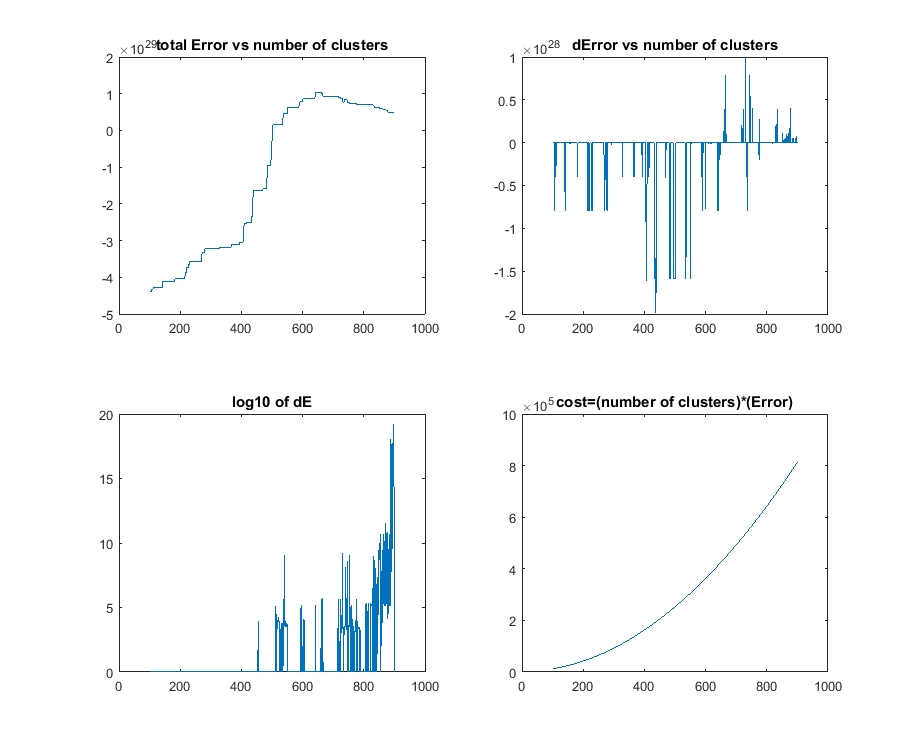
\includegraphics[width=\textwidth,height=300pt]{avg_fw_results.png}}
\clearpage
\boxed{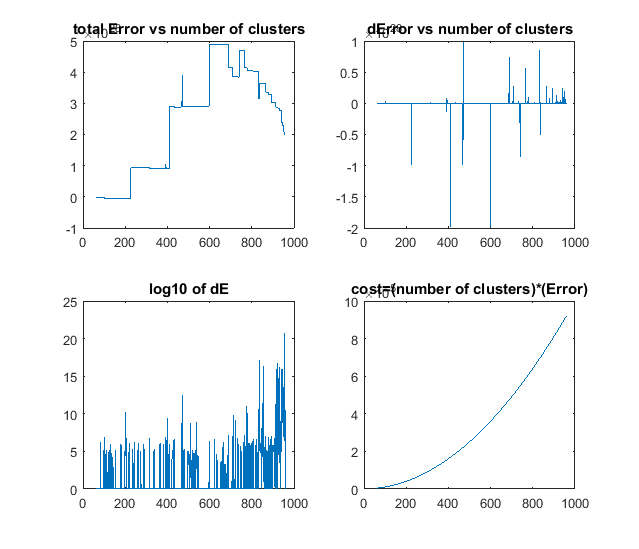
\includegraphics[width=\textwidth,height=250pt]{avg_acl_results.png}}
\clearpage
\boxed{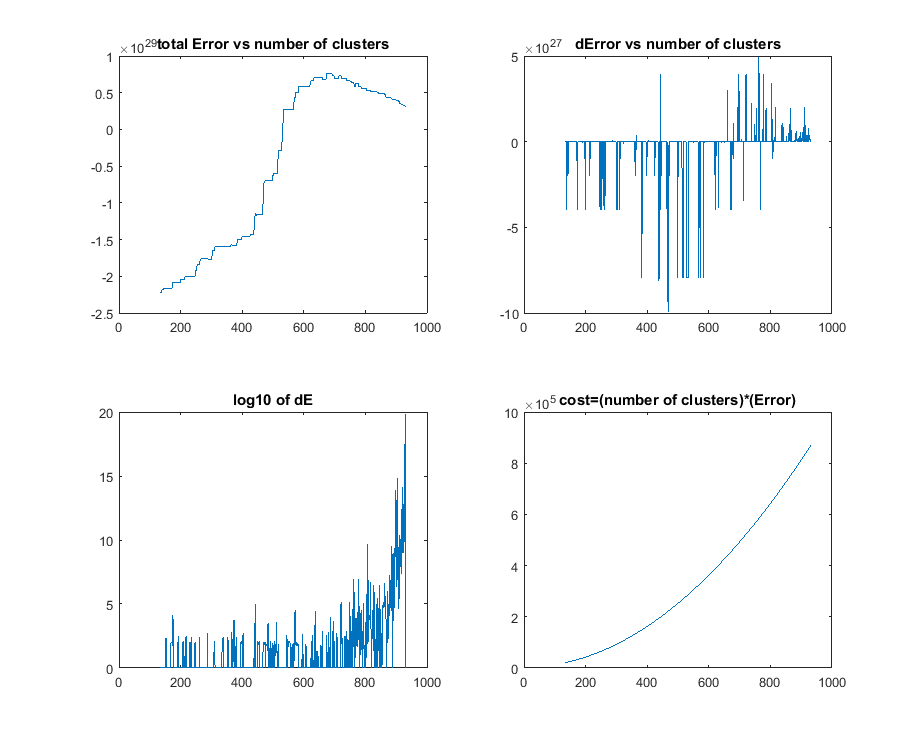
\includegraphics[width=\textwidth,height=250pt]{total_avg.png}}
\clearpage
\boxed{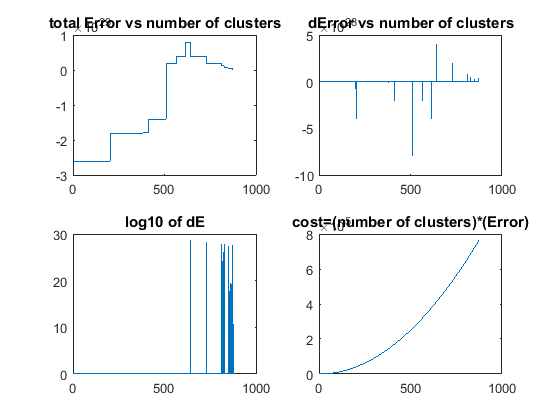
\includegraphics[width=\textwidth,height=250pt]{fw_seed_1000.png}}
\clearpage
\boxed{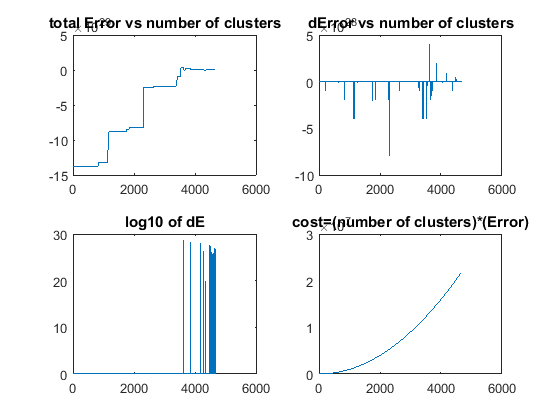
\includegraphics[width=\textwidth,height=350pt]{fw1_seed_5000.png}}
\end{widetext}
\end{document}
